\documentclass{standalone}
\usepackage{tikz}
\usepackage{ctex,siunitx}
\usepackage{tkz-euclide}
\usepackage{amsmath}
\usetikzlibrary{patterns, calc}
\usetikzlibrary {decorations.pathmorphing, decorations.pathreplacing, decorations.shapes,}
\begin{document}
\small
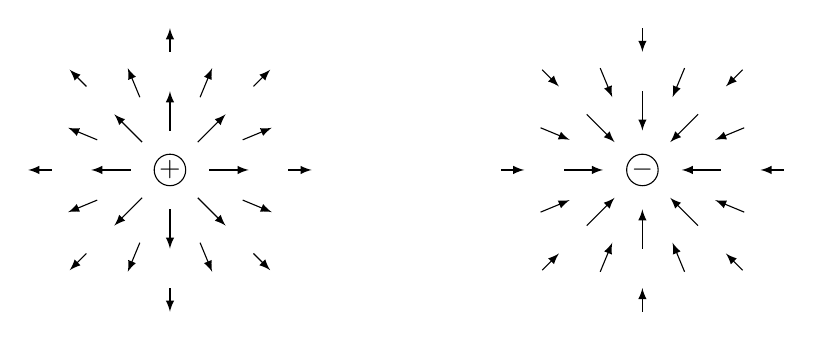
\begin{tikzpicture}[>=latex,scale=1.0]
  \draw(-3.0,0)circle(0.2)node{$+$};
  \draw(3.0,0)circle(0.2)node{$-$};
  \foreach \x in {0,45,...,315}
  {
    \draw[->]([shift=(\x:0.5)]-3.0,0)--++(\x:0.5);
    \draw[->]([shift=(\x:1.5)]-3.0,0)--++(\x:0.3);
    \draw[->]([shift=(\x+22.5:1.0)]-3.0,0)--++(\x+22.5:0.4);
    \draw[<-]([shift=(\x:0.5)]3.0,0)--++(\x:0.5);
    \draw[<-]([shift=(\x:1.5)]3.0,0)--++(\x:0.3);
    \draw[<-]([shift=(\x+22.5:1.0)]3.0,0)--++(\x+22.5:0.4);
  }
\end{tikzpicture}
\end{document}